\section{First chapter}
As said in Section \ref{sec:introduction}, this is just an example. This is a very good one, indeed, it has also subsections and images!

\subsection{Subsection example} 
\label{sec:subection-example}
It is pretty easy to make subsections and add images in latex. And everything can have a label that we can use when we make references in the text. 

For example, have a look at Figure \ref{fig:atari-pong}, which is a screenshot of an Atari game.

\begin{figure}[ht]
	\centering
	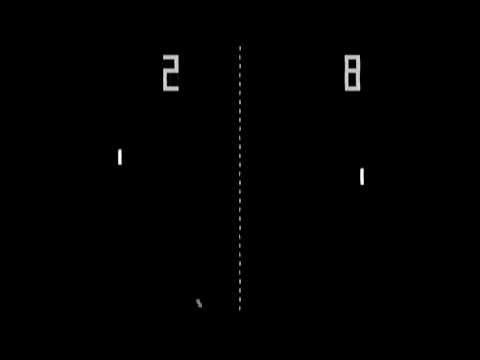
\includegraphics[width=0.4\textwidth]{img/atari-pong}
	\label{fig:atari-pong}
	\caption{Atari pong, a very popular game in the past years.}
\end{figure}

\subsection{New lines and indentations}

Latex automatically adds spaces between paragraphs and manages indentation.One can customize the default behavior, which is to indent for every new paragraph. 

Like this one. In the code, you just need to have a blank space between two lines to start a new paragraph.

This line, for instance, is the starting of yet another paragraph.

\subsection*{Not-numbered sections}
All sections end up in the table of contents if we decide to display it by adding \texttt{\textbackslash tableofcontents} at the beginning of the document. If we put an an asterisk (*) before the title of the section, it does not appear in the table of contents.

This sub-section, for instance, is not numbered and it does not appear in the contents.
 